% -*- coding: utf-8 -*-
\documentclass[UTF8,a4paper,10pt]{ctexart}

\usepackage[left=3.17cm, right=3.17cm, top=2.74cm, bottom=2.74cm]{geometry}
\usepackage{amsmath}
\usepackage{amssymb}
\usepackage{graphicx,subfig}
\usepackage{float}
\usepackage{caption}
\usepackage{enumerate}
\usepackage{booktabs}
\usepackage{multirow}
\usepackage{array}
\usepackage{longtable}
\usepackage[colorlinks=true,linkcolor=black,citecolor=black,urlcolor=blue]{hyperref}
\usepackage{xcolor}
\usepackage{listings}
\usepackage{fancyhdr}
\usepackage{algorithm}
\usepackage{algorithmicx}
\usepackage{algpseudocode}
\usepackage{enumitem}
\usepackage{pifont}
\usepackage{tikz}
\usepackage{eso-pic}
\usepackage{framed}

\graphicspath{{../src/}}

\newcommand{\tabincell}[2]{\begin{tabular}{@{}#1@{}}#2\end{tabular}}

\newcommand{\yihao}{\fontsize{26pt}{36pt}\selectfont}
\newcommand{\erhao}{\fontsize{22pt}{28pt}\selectfont}
\newcommand{\xiaoer}{\fontsize{18pt}{18pt}\selectfont}
\newcommand{\sanhao}{\fontsize{16pt}{24pt}\selectfont}
\newcommand{\xiaosan}{\fontsize{15pt}{22pt}\selectfont}
\newcommand{\sihao}{\fontsize{14pt}{21pt}\selectfont}
\newcommand{\banxiaosi}{\fontsize{13pt}{19.5pt}\selectfont}
\newcommand{\xiaosi}{\fontsize{12pt}{18pt}\selectfont}
\newcommand{\dawuhao}{\fontsize{11pt}{11pt}\selectfont}
\newcommand{\wuhao}{\fontsize{10.5pt}{15.75pt}\selectfont}

\ctexset{
  section = {
    format = \bfseries\zihao{4},
    name = {,、},
    number = \chinese{section}
  },
  subsection = {
    format = \bfseries\zihao{-4},
    name = {（,）},
    number = \chinese{subsection}
  },
  subsubsection = {
    format = \bfseries\zihao{5},
    number = \arabic{subsubsection}
  }
}

\pagestyle{fancy}
\lhead{\kaishu 数据安全课程作业}
\chead{基于 zkSNARK 的零知识证明实验}
\rhead{\kaishu 2312309\ 祝铭堃}
\lfoot{}
\cfoot{\thepage}
\rfoot{}
\renewcommand{\headrulewidth}{0.1pt}
\renewcommand{\footrulewidth}{0pt}
\setlength{\headheight}{15pt}

\newcommand{\HRule}{\rule{\linewidth}{0.5mm}}
\newcommand{\HRulegrossa}{\rule{\linewidth}{1.2mm}}

\floatname{algorithm}{Algorithm}
\renewcommand{\algorithmicrequire}{\textbf{Input:}}
\renewcommand{\algorithmicensure}{\textbf{Output:}}

\lstset{
breaklines,
basicstyle=\small\ttfamily,
escapeinside=``,
keywordstyle=\color{blue!70}\bfseries,
commentstyle=\color{red!50!green!50!blue!50},
stringstyle=\ttfamily,
showstringspaces=false,
extendedchars=false,
linewidth=\textwidth,
numbers=left,
numberstyle=\tiny\color{blue!50},
frame=trbl,
rulesepcolor=\color{red!20!green!20!blue!20}
}

\newcommand{\cmark}{\ding{51}}
\newcommand{\xmark}{\ding{55}}
\newcommand{\done}{\rlap{$\square$}{\raisebox{2pt}{\large\hspace{1pt}\cmark}}\hspace{-2.5pt}}
\newcommand{\wontfix}{\rlap{$\square$}{\large\hspace{1pt}\xmark}}

\newcommand{\watermark}[3]{\AddToShipoutPictureBG{
\parbox[b][\paperheight]{\paperwidth}{
\vfill
\centering
\tikz[remember picture, overlay]
  \node [rotate = #1, scale = #2] at (current page.center)
    {\textcolor{gray!80!cyan!30!magenta!30}{#3}};
\vfill}}}

\newcommand{\screenshotplaceholder}[2]{
\begin{figure}[H]
    \centering
    \fbox{
    \begin{minipage}[c][5.0cm][c]{0.84\textwidth}
        \centering
        \textbf{#1}\\[0.8em]
        #2
    \end{minipage}}
    \caption{#1}
\end{figure}
}

\newcommand{\reportfigure}[3]{
\IfFileExists{../src/#2}{
\begin{figure}[H]
    \centering
    \includegraphics[width=0.95\textwidth,height=0.72\textheight,keepaspectratio]{../src/#2}
    \caption{#1}
\end{figure}
}{
\screenshotplaceholder{#1}{#3}
}
}

\begin{document}
\renewcommand{\contentsname}{目录}
\renewcommand{\figurename}{图}
\renewcommand{\tablename}{表}
\renewcommand{\today}{\number\year 年 \number\month 月 \number\day 日}

\begin{titlepage}
    \begin{center}
    
\includegraphics[width=0.8\textwidth]{NKU.png}\\[1cm]
    \vspace{20mm}
    {\Huge \heiti 南开大学}\\[0.9cm]
    {\huge \heiti 网络空间安全学院}\\[0.9cm]
    {\Large \textbf{《数据安全》课程作业}}\\[0.8cm]
    \HRule \\[0.9cm]
    {\LARGE \bfseries 基于 zkSNARK 的零知识证明实验}\\[0.4cm]
    \HRule \\[2.0cm]
    \vspace{\fill}
    \centering
    {\LARGE 姓名\ :\ 祝铭堃}\\[0.5cm]
    {\LARGE 学号\ :\ 2312309}\\[0.5cm]
    {\LARGE 专业\ :\ 计算机科学与技术}\\[0.5cm]
    {\LARGE 指导教师\ :\ 刘哲理}\\[0.5cm]
    \vfill
    {\Large \today}
    \end{center}
\end{titlepage}

\newpage
\tableofcontents

\newpage
\watermark{60}{10}{NKU}
\setcounter{page}{1}

\section{实验要求}
本次实验题目为“零知识证明实践”。需要参考教材第四章及实验 3.1 的思路，完成如下命题的证明生成与验证：
\[
x^3 + x + 5 = Out.
\]

其中，$Out$ 为公开输入，默认取值为 $35$；证明者持有私密解 $x$，在默认演示中使用 $x=3$。实验目标是让验证者相信证明者知道一个满足约束的解，同时不直接暴露该解本身。

结合题目要求与本次实现过程，我们在正式开始实验之前进一步明确了以下边界条件：
\begin{itemize}
    \item 证明系统采用教材第四章介绍的 zkSNARK 路线，底层使用算术电路与 R1CS 描述命题；
    \item 证明与验证通过 \texttt{setup / prove / verify} 三阶段完成；
    \item 完整实验目录与构建工作区均保留在 WSL 中，前者保存代码、脚本、结果与报告，后者隔离外部依赖与编译产物；
    \item 若在 WSL 中使用 Python，则统一通过 \texttt{conda} 环境管理，不直接依赖系统 Python 安装实验辅助依赖。
\end{itemize}

\section{项目结构与仓库说明}
本次实验的代码、脚本、结果与报告统一组织在本地课程目录下，我们将目录划分如下：
\begin{itemize}
    \item \texttt{实验/lab2/zk\_lab/}：libsnark 证明代码；
    \item \texttt{实验/lab2/scripts/}：WSL shell 脚本与环境辅助脚本；
    \item \texttt{实验/lab2/results/}：证明密钥、验证密钥、证明文件与日志；
    \item \texttt{实验/lab2/report/}：LaTeX 报告；
    \item \texttt{实验/lab2/src/}：运行截图与补充材料。
\end{itemize}

本实验对应的 GitHub 仓库为 \href{https://github.com/EricEvans-e/data_security2026}{\texttt{EricEvans-e/data\_security2026}}。

当前报告对应的实验内容位于该仓库的 \texttt{实验/lab2/} 目录下，我们后续展示的代码、脚本、结果文件与截图说明均以该目录中的实际内容为准。

\section{实验原理}

\subsection{零知识证明的基本思想}
零知识证明（Zero-Knowledge Proof, ZKP）允许证明者在不泄露秘密本身的前提下，使验证者相信某个公开命题成立。教材中给出的定义可以概括为：证明者知道一个使得公开谓词 $C(x)=1$ 的秘密输入 $x$，并向验证者证明“自己确实知道它”，而不是把该秘密直接交给验证者。

零知识证明通常强调以下三个性质：
\begin{itemize}
    \item \textbf{完备性}：若证明者确实知道合法见证，验证应当以高概率成功；
    \item \textbf{可靠性}：若证明者不知道见证，则伪造证明应当非常困难；
    \item \textbf{零知识性}：验证者只能获得“命题成立”这一事实，而不能得到关于见证本身的额外信息。
\end{itemize}

\subsection{zkSNARK 与 libsnark}
zkSNARK 是一类典型的非交互式零知识证明技术，特点是证明短、验证快且适合公开验证。教材示例中使用 \texttt{libsnark} 框架来完成开发，该框架提供了：
\begin{itemize}
    \item 约束系统定义；
    \item 证明密钥与验证密钥生成；
    \item 证明构造；
    \item 证明验证。
\end{itemize}

在工程上，我们按照如下流程完成本实验：
\begin{enumerate}
    \item 将待证明命题转成算术电路；
    \item 将算术电路写成 R1CS 约束；
    \item 在 \texttt{setup} 阶段生成 \texttt{pk.raw} 和 \texttt{vk.raw}；
    \item 在 \texttt{prove} 阶段使用见证构造 \texttt{proof.raw}；
    \item 在 \texttt{verify} 阶段使用公开输入和验证密钥检查证明是否成立。
\end{enumerate}

这三个阶段在语义上也有明确分工。\texttt{setup} 负责把“约束系统”转化为后续可复用的证明参数；\texttt{prove} 负责把私有见证代入约束系统，并构造满足该系统的证明；\texttt{verify} 则只接收公开输入、验证密钥和证明文件，不再接触见证本身。也正因为这种分工，实验中的“知道解但不公开解”才能在代码层面落到可执行流程上，而不只是停留在概念描述。

\subsection{算术电路与 R1CS 约束}
本实验证明的命题是
\[
x^3 + x + 5 = Out.
\]
为了使用 zkSNARK，需要将其拆成仅包含加法和乘法的中间变量形式。设中间量如下：
\[
x\_square = x \cdot x,
\]
\[
x\_cube = x\_square \cdot x,
\]
\[
sum\_with\_x = x\_cube + x,
\]
\[
expr\_out = sum\_with\_x + 5.
\]

最后要求：
\[
expr\_out = Out.
\]

因此，本实验对应的 R1CS 约束固定为表 \ref{tab:r1cs} 所示。

\begin{table}[H]
    \centering
    \begin{tabular}{cl}
        \toprule
        编号 & 约束 \\
        \midrule
        C1 & $x \cdot x = x\_square$ \\
        C2 & $x\_square \cdot x = x\_cube$ \\
        C3 & $(x\_cube + x)\cdot 1 = sum\_with\_x$ \\
        C4 & $(sum\_with\_x + 5)\cdot 1 = expr\_out$ \\
        C5 & $expr\_out \cdot 1 = Out$ \\
        \bottomrule
    \end{tabular}
    \caption{实验命题对应的 R1CS 约束}
    \label{tab:r1cs}
\end{table}

在本实现中：
\begin{itemize}
    \item 公有输入只有一个：\texttt{out}；
    \item 私有见证包括：\texttt{x}、\texttt{x\_square}、\texttt{x\_cube}、\texttt{sum\_with\_x}、\texttt{expr\_out}。
\end{itemize}

这种划分与实验目标是完全一致的。验证者真正需要知道的只有“公开命题是否成立”，也就是 $Out$ 的值；而为了证明该命题成立所必需的中间量，全部被纳入私有见证。这样一来，验证阶段既能利用约束系统检查证明的正确性，又不会直接接触原始秘密输入 $x$ 及其展开过程。

\subsection{默认示例的见证计算}
当默认示例取 $x=3$ 时，可得到：
\[
x\_square = 3^2 = 9,
\quad
x\_cube = 3^3 = 27,
\]
\[
sum\_with\_x = 27 + 3 = 30,
\quad
expr\_out = 30 + 5 = 35.
\]
因此在默认演示下，公开输入确实可以设为 $Out=35$，验证者只看到公开输入和证明文件，不需要获得 $x=3$ 本身。

选择这个默认示例还有一个实际好处：所有中间量都较小，便于我们手工核对日志中的 witness 展开结果。以 \texttt{prove\_valid.log} 为例，当日志中出现 \texttt{3, 9, 27, 30, 35} 这一序列时，我们就能够快速判断代码中的见证构造、约束连接和公开输入设置是一致的。

\section{实验过程}

\subsection{实验环境与工作目录设计}
本实验最终的环境准备、编译、运行、截图和结果整理全部在 WSL 中完成。为了既保留一份完整的实验目录，又避免把庞大的 \texttt{libsnark} 源码树和编译产物直接混入实验代码目录，我们在 WSL 内将目录划分为“完整实验目录”和“构建工作区”两个层次。

WSL 中的完整实验目录为：
\begin{lstlisting}[title=WSL 侧完整实验目录,frame=trbl]
/home/eric/workspace/lab2/
|- zk_lab/
|- scripts/
|- results/
|- report/
|- src/
`- tests/
\end{lstlisting}

其中 \texttt{zk\_lab/} 保存证明程序源码，\texttt{scripts/} 保存环境初始化、编译与运行脚本，\texttt{results/}、\texttt{src/} 和 \texttt{report/} 分别用于存放结果、截图和实验报告。

为避免将外部依赖与构建产物混入上述目录，我们另外准备了 WSL 构建工作区：
\begin{lstlisting}[title=WSL 侧构建工作区,frame=trbl]
/home/eric/workspace/data-security-lab2/
|- env/
|- libsnark-src/
|- build/
|- artifacts/
`- logs/
\end{lstlisting}

\reportfigure{WSL 独立工作目录创建成功}{01-wsl-workspace.png}{此处插入图 1：展示 \texttt{/home/eric/workspace/data-security-lab2/} 及其子目录已经创建完成。}

这张图主要用来说明 WSL 侧工作区已经按照预期创建完成，为后续编译和运行提供了固定目录。

\subsection{conda 环境与 libsnark 环境初始化}
考虑到用户要求“WSL 中如果使用 Python，则建议用 conda 管理环境”，我们在初始化脚本中固定创建环境 \texttt{datasec-lab2-zk}。即使主证明程序使用 C++/libsnark，辅助检查、日志整理和后续可扩展脚本也统一在该环境内运行。这样，我们在整理日志和后续复现实验时会更加方便。

以下命令均在 \path{/home/eric/workspace/lab2/} 根目录中执行。为便于复现，我们先固定构建工作区变量，再调用初始化脚本：
\begin{lstlisting}[title=初始化 WSL 环境,frame=trbl]
cd /home/eric/workspace/lab2
WORKSPACE_ROOT=/home/eric/workspace/data-security-lab2
sh ./scripts/wsl_setup_env.sh "$PWD" "$WORKSPACE_ROOT"
\end{lstlisting}

这条命令是整个 WSL 实验环境准备的入口，后续所需的完整实验目录、构建工作区、Conda 环境和依赖软件都会通过它统一完成初始化。

该脚本内部会依次完成以下工作：
\begin{enumerate}
    \item 修正 WSL 中异常的 \texttt{HOME} 环境变量；
    \item 安装 \texttt{build-essential}、\texttt{cmake}、\texttt{git} 等系统依赖；
    \item 安装 Miniconda；
    \item 创建 \texttt{datasec-lab2-zk} 环境；
    \item 在 WSL 构建工作区中准备 \texttt{libsnark\_abc} 及其子模块，形成后续编译所需的依赖目录。
\end{enumerate}

本次实际运行完成后，\texttt{env/environment.txt} 中记录的关键环境信息如下。通过这些信息，我们可以确认操作系统、Conda 环境以及 libsnark 工作目录都已经准备完成：
\begin{lstlisting}[title=WSL 环境摘要,frame=trbl]
OS_PRETTY_NAME=Ubuntu 22.04.5 LTS
GENERATED_AT=2026-04-21 18:05:57 CST
HOME=/home/eric
WORKSPACE_ROOT=/home/eric/workspace/data-security-lab2
CONDA_ROOT=/home/eric/miniconda3
CONDA_ENV_NAME=datasec-lab2-zk
CONDA_PYTHON=/home/eric/miniconda3/envs/datasec-lab2-zk/bin/python
PYTHON_VERSION=Python 3.10.20
GIT=/usr/bin/git
CMAKE=/usr/bin/cmake
CXX=/usr/bin/c++
LIBSNARK_ROOT=/home/eric/workspace/data-security-lab2/libsnark-src/libsnark_abc-master
\end{lstlisting}

\reportfigure{conda 环境创建与激活}{02-conda-env.png}{此处插入图 2：展示 \texttt{datasec-lab2-zk} 环境创建完成，或 \texttt{conda} 环境信息输出。}

从这张图中可以看到，\texttt{datasec-lab2-zk} 环境已经能够正常激活，且 \texttt{which python} 的输出明确指向对应虚拟环境中的解释器，说明后续测试与辅助脚本会在统一环境中运行。

\reportfigure{libsnark 环境准备成功}{03-libsnark-ready.png}{此处插入图 3：展示 \texttt{libsnark\_abc-master} 已经拉取完成，并具备后续编译条件。}

这张图展示了 \texttt{environment.txt} 中记录的环境摘要，其中包括 Ubuntu 版本、Python 版本以及 \texttt{LIBSNARK\_ROOT} 路径。它不仅说明外部依赖源码已经准备完成，也说明后续编译所需的路径信息已经被固定下来。

\subsection{证明代码实现}
证明代码放在 \texttt{zk\_lab/} 目录。我们实现时使用的核心文件如下：
\begin{itemize}
    \item \texttt{common.hpp}：定义曲线类型、约束系统、见证结构、序列化辅助函数；
    \item \texttt{zk\_setup.cpp}：生成证明密钥与验证密钥；
    \item \texttt{zk\_prove.cpp}：根据给定见证生成证明；
    \item \texttt{zk\_verify.cpp}：读取验证密钥与证明文件，完成验证。
\end{itemize}

\texttt{common.hpp} 中的实现重点是：我们先在 \texttt{protoboard} 上分配公有输入和私有变量，再按表 \ref{tab:r1cs} 依次加入约束。这样在 \texttt{setup / prove / verify} 三个阶段都可以复用同一套电路定义。

\subsection{关键代码展示}
结合往年实验报告的写法，我们在本报告中补充展示三段最能体现本实验核心逻辑的代码，分别对应“见证计算与约束构造”“证明生成”“证明验证”三个环节。

\begin{lstlisting}[title=关键代码 1：见证计算与 R1CS 约束构造,language=C++,frame=trbl]
inline WitnessValues build_witness(const long long x)
{
    WitnessValues witness{};
    witness.x = x;
    witness.x_square = x * x;
    witness.x_cube = witness.x_square * x;
    witness.sum_with_x = witness.x_cube + x;
    witness.expr_out = witness.sum_with_x + 5;
    return witness;
}

template<typename Field>
inline libsnark::protoboard<Field> build_protoboard(
    const long long public_out,
    const WitnessValues *witness = nullptr)
{
    libsnark::protoboard<Field> pb;
    ...
    pb.set_input_sizes(1);
    pb.val(out) = Field(public_out);

    pb.add_r1cs_constraint(libsnark::r1cs_constraint<Field>(x, x, x_square));
    pb.add_r1cs_constraint(libsnark::r1cs_constraint<Field>(x_square, x, x_cube));
    pb.add_r1cs_constraint(libsnark::r1cs_constraint<Field>(x_cube + x, 1, sum_with_x));
    pb.add_r1cs_constraint(libsnark::r1cs_constraint<Field>(sum_with_x + 5, 1, expr_out));
    pb.add_r1cs_constraint(libsnark::r1cs_constraint<Field>(expr_out, 1, out));
    ...
}
\end{lstlisting}

这段代码是整个证明系统的基础，它负责把私有见证和公开命题组织到同一套约束系统中。

上述代码首先根据秘密输入 \texttt{x} 展开中间见证值，然后我们在 \texttt{protoboard} 上依次加入 5 条 R1CS 约束。其中 \texttt{pb.set\_input\_sizes(1)} 明确规定只有 \texttt{out} 属于公有输入，其余变量均作为私有见证参与证明。
这部分代码摘自 \path{zk_lab/common.hpp}，对应实验中电路建模与约束复用的公共实现。

\begin{lstlisting}[title=关键代码 2：证明阶段的 witness 检查与 proof 生成,language=C++,frame=trbl]
const auto witness = lab2::build_witness(x_value);

if (!lab2::witness_matches_statement(witness, out_value)) {
    std::cerr << "Witness does not satisfy the public statement." << std::endl;
    return EXIT_FAILURE;
}

const auto pb = lab2::build_protoboard<lab2::FieldT>(out_value, &witness);
if (!pb.is_satisfied()) {
    std::cerr << "Constraint system is not satisfied." << std::endl;
    return EXIT_FAILURE;
}

const auto proof = libsnark::r1cs_gg_ppzksnark_prover<lab2::ppT>(
    pk,
    pb.primary_input(),
    pb.auxiliary_input());
\end{lstlisting}

这段代码体现了证明阶段最关键的逻辑，也就是先检查 witness，再根据满足约束的输入生成证明文件。只有 witness 与公开命题一致、并且完整约束系统满足时，我们才会调用 \texttt{prover} 生成 \texttt{proof.raw}。
这部分代码摘自 \path{zk_lab/zk_prove.cpp}，对应实验中证明生成程序的核心逻辑。

\begin{lstlisting}[title=关键代码 3：验证阶段的核心调用,language=C++,frame=trbl]
const auto pb = lab2::build_protoboard<lab2::FieldT>(out_value, nullptr);
const bool verified = libsnark::r1cs_gg_ppzksnark_verifier_strong_IC<lab2::ppT>(
    vk,
    pb.primary_input(),
    proof);

std::cout << "Verification result: " << (verified ? 1 : 0) << std::endl;
\end{lstlisting}

这段代码展示了验证阶段的核心调用方式，即只依赖公开输入、验证密钥和证明文件完成最终检查。

验证阶段不再接触私有 witness，而是只使用验证密钥、公开输入和证明文件完成检查。这也是我们在本实验中能够体现“公开验证而不泄露秘密”的关键所在。
这部分代码摘自 \path{zk_lab/zk_verify.cpp}，对应实验中验证程序的核心入口。

\subsection{编译流程}
编译命令如下：
\begin{lstlisting}[title=编译证明程序,frame=trbl]
cd /home/eric/workspace/lab2
WORKSPACE_ROOT=/home/eric/workspace/data-security-lab2
sh ./scripts/wsl_build_lab2.sh "$PWD" "$WORKSPACE_ROOT"
\end{lstlisting}

我们通过这条命令统一触发源码同步、CMake 编译和日志回收三个步骤。

该脚本会：
\begin{enumerate}
    \item 将 \texttt{zk\_lab/} 中的源码同步到 WSL 工作区中的 \texttt{libsnark\_abc-master/src/}；
    \item 在外部 bundle 的 \texttt{src/CMakeLists.txt} 中追加 \texttt{zk\_setup}、\texttt{zk\_prove}、\texttt{zk\_verify} 三个目标；
    \item 调用 CMake 完成编译；
    \item 将生成日志拷回 \texttt{results/logs/build.log}。
\end{enumerate}

编译完成后，WSL 工作区中能够看到 \texttt{zk\_setup}、\texttt{zk\_prove} 和 \texttt{zk\_verify} 三个目标程序，这说明后续 setup、prove 和 verify 的执行入口已经准备完成。

\begin{figure}[H]
    \centering
    
\includegraphics[width=0.9\textwidth]{../src/6.png}
    
    \smallskip
    
    （a）WSL 中执行编译脚本并输出完成提示
    
    \vspace{0.8em}
    
    
\includegraphics[width=0.9\textwidth]{../src/7.png}
    
    \smallskip
    
    （b）编译后生成的三个可执行文件
    
    \caption{编译阶段的终端输出与产物检查}
\end{figure}

这组图片分别展示了编译脚本执行完成时的终端输出，以及编译结束后生成的三个目标程序，可以更直观地说明构建流程已经真正落到了可执行产物上。

\subsection{正确样例运行流程}
默认演示采用公开输入 \texttt{Out=35} 和私密输入 \texttt{x=3}。首先，我们在 \path{/home/eric/workspace/lab2/} 目录执行如下 WSL 命令：
\begin{lstlisting}[title=运行正确样例,frame=trbl]
cd /home/eric/workspace/lab2
WORKSPACE_ROOT=/home/eric/workspace/data-security-lab2
sh ./scripts/wsl_run_demo.sh "$PWD" "$WORKSPACE_ROOT" 3 35
\end{lstlisting}

这条命令会顺序执行 setup、prove 和 verify 三个阶段，用于验证默认样例是否能够完整跑通。

内部执行顺序为：
\begin{enumerate}
    \item \texttt{zk\_setup --artifacts-dir ... --out 35}
    \item \texttt{zk\_prove --artifacts-dir ... --x 3 --out 35}
    \item \texttt{zk\_verify --artifacts-dir ... --out 35}
\end{enumerate}

本次运行会在 \texttt{results/artifacts/} 和 \texttt{results/logs/} 下生成对应的密钥、证明文件与日志，后文主要结合日志内容和运行截图分析其正确性。

结合本次真实运行日志与后续截图，可以提取出以下关键结果：
\begin{itemize}
    \item \texttt{setup} 阶段成功生成 \texttt{pk.raw} 与 \texttt{vk.raw}，约束数量为 5，公开输入规模为 1；
    \item \texttt{prove} 阶段在 \texttt{x=3} 条件下得到 \texttt{x\_square=9}、\texttt{x\_cube=27}、\texttt{sum\_with\_x=30}、\texttt{expr\_out=35}，并成功写出 \texttt{proof.raw}；
    \item \texttt{verify} 阶段输出 \texttt{Verification result: 1}，说明验证者接受了该证明。
\end{itemize}

\reportfigure{正确样例脚本执行完成}{8.png}{此处插入补充截图：展示 \texttt{wsl\_run\_demo.sh} 执行结束并输出 \texttt{Valid demo finished}。}

这张图对应正确样例总控脚本执行完成后的状态，说明 setup、prove 和 verify 三个阶段已经被顺序跑通。

\reportfigure{zk\_setup 生成密钥}{04-setup.png}{此处插入图 4：展示 \texttt{setup.log} 中密钥生成成功、约束数量和输出文件路径。}

这张图主要用于说明 setup 阶段已经成功生成 proving key 和 verification key，并记录了电路规模等关键信息。

\reportfigure{zk\_prove 成功生成证明}{05-prove-valid.png}{此处插入图 5：展示 \texttt{prove\_valid.log} 中 witness、primary input 和证明生成完成的信息。}

这张图展示了正确 witness 条件下证明生成成功的日志内容，可以和前面的 witness 展开结果对应起来。同时，日志中给出的 \texttt{Primary input} 与 \texttt{Auxiliary input} 也说明公开输入和私有见证已经被正确分离。

\begin{figure}[H]
    \centering
    \subfloat[终端输出中的 \texttt{Verification result: 1}]{
        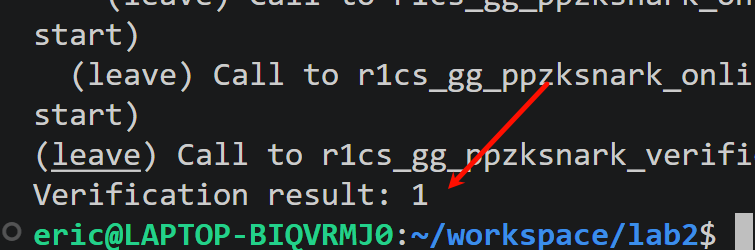
\includegraphics[width=0.48\textwidth]{../src/06-verify-valid.png}
    }
    \hfill
    \subfloat[\texttt{verify\_valid.log} 文件视图中的公开输入与验证结果]{
        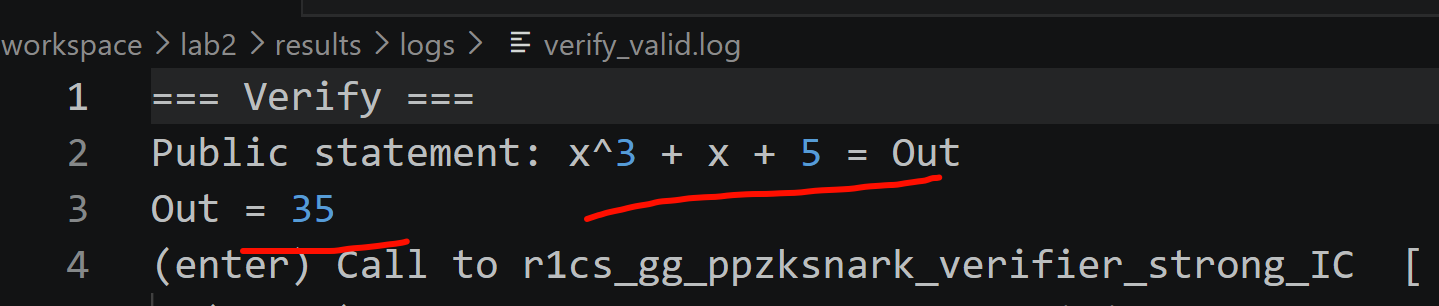
\includegraphics[width=0.48\textwidth]{../src/17.png}
    }
    \caption{zk\_verify 验证结果为 1}
\end{figure}

这组图片分别从终端输出和日志文件视图两个角度展示了正确样例的最终验证结果。前者直接给出 \texttt{Verification result: 1}，后者补充了公开输入 \texttt{Out = 35} 与日志上下文，因此可以更完整地说明验证者已经在不知道秘密输入的情况下接受了该证明。

\subsection{错误样例运行流程}
为了验证系统的可靠性，我们还执行了两个负样例：
\begin{enumerate}
    \item 错误 witness：令 \texttt{x=4}、\texttt{out=35}，则约束不成立，证明阶段应失败；
    \item 错误公开输入：先用 \texttt{x=3}、\texttt{out=35} 生成合法证明，再用 \texttt{out=36} 验证，结果应失败。
\end{enumerate}

在 WSL 中执行的负样例命令如下：
\begin{lstlisting}[title=运行负样例,frame=trbl]
cd /home/eric/workspace/lab2
WORKSPACE_ROOT=/home/eric/workspace/data-security-lab2
sh ./scripts/wsl_run_negative_cases.sh "$PWD" "$WORKSPACE_ROOT"
\end{lstlisting}

通过这个脚本，我们可以一次性验证错误 witness 和错误公开输入两种负样例。

结合本次实际运行日志，可以提炼出两个关键负样例结论：当 \texttt{x=4, out=35} 时，证明阶段会先算出 \texttt{expr\_out=73}，随后直接给出 \texttt{Witness does not satisfy the public statement.}；当使用合法证明文件但把公开输入改为 \texttt{out=36} 时，验证阶段输出 \texttt{Verification result: 0}。这两个结果分别对应“错误见证无法生成证明”和“错误公开输入无法通过验证”。

\reportfigure{负样例脚本执行完成}{12.png}{此处插入补充截图：展示 \texttt{wsl\_run\_negative\_cases.sh} 执行结束并输出 \texttt{Negative cases finished}。}

这张图说明负样例总控脚本已经顺利执行完成，便于我们确认两类错误场景都被完整覆盖。

\reportfigure{错误 witness 被拒绝}{07-prove-invalid.png}{此处插入图 7：展示 \texttt{prove\_invalid.log} 中 witness 不满足公开命题或约束系统不满足的提示。}

这张图展示了错误 witness 在证明阶段就被系统拒绝的结果，说明证明者不能为不满足约束的输入构造合法证明。

\reportfigure{错误公开输入验证为 0}{08-verify-wrong-out.png}{此处插入图 8：展示 \texttt{verify\_wrong\_out.log} 中验证失败的结果。}

这张图则说明即使证明文件本身来自一次合法生成，只要验证时替换了公开输入，验证结果仍然会失败。

\section{实验结果与分析}

\subsection{结果文件}
从 WSL 构建工作区同步回完整实验目录的结果文件位于：
\begin{itemize}
    \item \texttt{results/artifacts/}
    \item \texttt{results/logs/}
\end{itemize}

这些文件分别对应 \texttt{setup}、\texttt{prove}、\texttt{verify} 三个阶段及其负样例运行日志，便于直接引用到报告或后续答辩展示中。

\begin{table}[H]
    \centering
    \begin{tabular}{lll}
        \toprule
        文件 & 大小（字节） & 说明 \\
        \midrule
        \texttt{pk.raw} & 1209 & proving key \\
        \texttt{vk.raw} & 1148 & verification key \\
        \texttt{proof.raw} & 137 & zkSNARK proof \\
        \texttt{build.log} & 63668 & 编译日志 \\
        \texttt{setup.log} & 6970 & setup 阶段日志 \\
        \texttt{prove\_valid.log} & 5754 & 正确 witness 证明日志 \\
        \texttt{verify\_valid.log} & 4835 & 正确公开输入验证日志 \\
        \texttt{prove\_invalid.log} & 176 & 错误 witness 日志 \\
        \texttt{verify\_wrong\_out.log} & 4876 & 错误公开输入验证日志 \\
        \bottomrule
    \end{tabular}
    \caption{本次实验整理得到的实际结果文件}
\end{table}

\begin{figure}[H]
    \centering
    \subfloat[结果文件已从 WSL 构建工作区同步到完整实验目录]{
        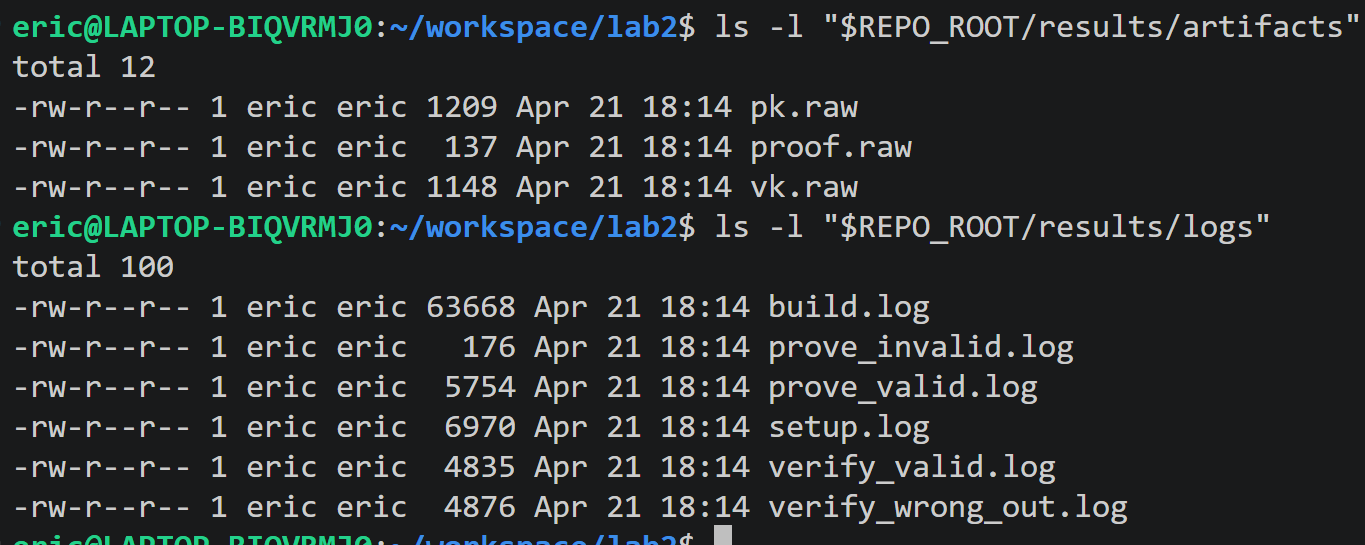
\includegraphics[width=0.48\textwidth]{../src/15.png}
    }
    \hfill
    \subfloat[在 conda 环境中执行 \texttt{pytest}，测试全部通过]{
        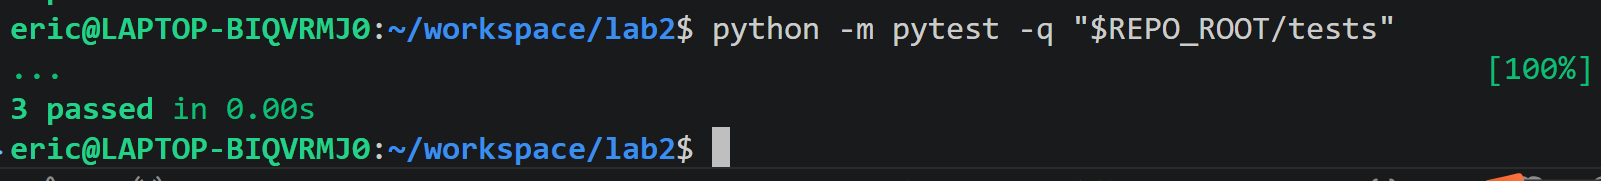
\includegraphics[width=0.48\textwidth]{../src/16.png}
    }
    \caption{实验结果文件检查与测试验证}
\end{figure}

这组图片展示了结果文件已经被成功同步回完整实验目录，同时测试脚本也已经在环境中运行通过，说明本次实验产物和自动化检查结果都已经整理完毕。

从文件大小也可以看到一些有代表性的现象：\texttt{proof.raw} 仅 137 字节，明显小于 \texttt{pk.raw} 和 \texttt{vk.raw}，这与 zkSNARK “证明短、便于传输”的特点是一致的；而 \texttt{prove\_invalid.log} 只有 176 字节，明显小于 \texttt{prove\_valid.log}，说明错误 witness 在证明阶段早早被拦截，没有进入完整的证明生成流程。

\subsection{正确样例分析}
对于正确样例 \texttt{x=3, out=35}，我们预期系统应呈现如下行为：
\begin{itemize}
    \item \texttt{setup} 阶段生成 \texttt{pk.raw} 与 \texttt{vk.raw}；
    \item \texttt{prove} 阶段先检查 witness 与公开命题一致，再构造证明 \texttt{proof.raw}；
    \item \texttt{verify} 阶段输出 \texttt{Verification result: 1}。
\end{itemize}

结合 \texttt{setup.log}、\texttt{prove\_valid.log} 与 \texttt{verify\_valid.log}，我们可以得到如下结论：
\begin{itemize}
    \item 电路中的约束数量为 5，与设计的 R1CS 约束完全一致；
    \item 公有输入规模为 1，正好对应唯一公开量 \texttt{Out}；
    \item 正确 witness 展开后得到的辅助输入依次为 \texttt{3, 9, 27, 30, 35}；
    \item 最终验证输出为 \texttt{1}，说明证明者确实可以在不公开 $x$ 的情况下，让验证者确认自己“知道一个使约束成立的见证”；
    \item 生成的 \texttt{proof.raw} 只有 137 字节，也从实验结果上体现了 zkSNARK 证明对象较短的特点。
\end{itemize}

从这个正确样例可以进一步看出，本实验中的“电路设计”“见证构造”“公开输入设置”三者是彼此严格对应的。首先，\texttt{setup.log} 中的 5 条约束正好对应表 \ref{tab:r1cs} 的五个关系；其次，\texttt{prove\_valid.log} 中依次出现的 \texttt{3, 9, 27, 30, 35}，又与我们在理论部分手工推导出的 witness 序列一致。也就是说，日志中的每一个中间值都能在前面的算术展开中找到来源，这说明代码实现并不是“黑箱地跑通了例子”，而是真的按照设计好的算术电路完成了约束编码。

另一方面，\texttt{verify} 阶段只接触公开输入 \texttt{Out=35}、验证密钥和证明文件，却依然能给出 \texttt{Verification result: 1}。这正是 zkSNARK 在本实验中最核心的效果：验证者并没有看到秘密输入 \texttt{x=3}，也没有直接访问中间变量，但仍然可以确信证明者掌握了一个满足约束系统的合法 witness。对于教学实验来说，这个结果把“零知识”和“可验证性”两个概念同时落到了可观察的日志输出上。

\subsection{负样例分析}
两个负样例分别说明：
\begin{itemize}
    \item 若 witness 自身不满足约束，则证明阶段就会被阻止，不能继续生成合法证明；
    \item 即使已经存在一份合法证明，只要公开输入发生变化，验证仍会失败。
\end{itemize}

更具体地说，我们可以从日志中看到：
\begin{itemize}
    \item 错误 witness 的日志直接输出 \texttt{Witness does not satisfy the public statement.}；
    \item 错误公开输入的日志输出 \texttt{Verification result: 0}，并伴随 \texttt{QAP divisibility check failed.}；
    \item \texttt{prove\_invalid.log} 很短，而 \texttt{verify\_wrong\_out.log} 与正确验证日志大小接近，说明前者在证明前置检查处提前退出，后者则完整执行了验证流程并在最终判定时失败。
\end{itemize}

因此，我们的实验同时展示了完备性与可靠性的直观效果。这样，我们就不仅验证了正确样例，也完成了对错误样例的对照分析。

这两个负样例其实分别卡在了系统的两个不同位置。第一个负样例中，问题出在证明者侧：当 \texttt{x=4} 时，程序会先算出 \texttt{expr\_out=73}，它与公开声明的 \texttt{Out=35} 不一致，因此证明流程在 witness 检查阶段就停止，不会继续生成一份看似“合法”的证明。第二个负样例中，问题则出在验证者侧：证明文件本身来自合法样例，但当公开输入被改成 \texttt{Out=36} 之后，验证过程会在最终一致性判断时拒绝这份证明。前者说明“错误见证无法伪造证明”，后者说明“合法证明也不能脱离原公开语句被复用”，两者合在一起，才构成了一套更完整的正确性与安全性展示。

\begin{table}[H]
    \centering
    \begin{tabular}{lll}
        \toprule
        场景 & 输入 & 预期结果 \\
        \midrule
        正确样例 & $x=3$, $Out=35$ & 验证通过，输出 1 \\
        错误 witness & $x=4$, $Out=35$ & 证明阶段失败 \\
        错误公开输入 & proof for $(3,35)$, verify with $Out=36$ & 验证失败，输出 0 \\
        \bottomrule
    \end{tabular}
    \caption{实验样例与预期输出}
\end{table}

\subsection{结果小结与复现性说明}
综合前面的日志、截图、测试与结果文件，可以把本次实验概括为一条完整且可重复执行的链路：先在 WSL 中完成环境初始化与 \texttt{libsnark} 依赖准备，再通过编译脚本生成 \texttt{zk\_setup}、\texttt{zk\_prove}、\texttt{zk\_verify} 三个可执行文件，随后分别运行正确样例与负样例脚本，最后把日志、二进制产物和截图整理回实验目录用于报告撰写。换句话说，本报告中的每一张关键截图，基本都能在 \texttt{results/logs/} 或 \texttt{results/artifacts/} 中找到对应的原始依据，而不是脱离代码与脚本单独整理出来的展示材料。

从复现角度看，这种组织方式也比较适合课程实验。环境准备、编译、正确样例、错误样例四个阶段，已经分别封装到 \texttt{wsl\_setup\_env.sh}、\texttt{wsl\_build\_lab2.sh}、\texttt{wsl\_run\_demo.sh} 和 \texttt{wsl\_run\_negative\_cases.sh} 中。后续如果需要重新截图、重新生成日志或重新核对某一项结果，只需要在同一工作区下重新执行对应脚本即可。这样既能保证报告中的分析有据可查，也能减少人工手动操作造成的路径错误、环境漂移或日志缺失问题。

因此，这次实验的意义不只是“成功跑通了一个 zkSNARK 示例”，更重要的是我们已经把该示例整理成了一套具有固定目录结构、固定运行脚本、固定输出位置的可复现实验流程。对于后续继续扩展更复杂的约束系统、替换不同的公开输入、或者进一步观察证明文件与日志行为变化，这套基础工作流都可以直接复用。

\section{实验心得与体会}
通过本次实验，我们可以更加直观地认识到 zkSNARK 的工程实现并不是直接对原始数学公式做证明，而是需要先把命题拆解为算术电路，再进一步转化为标准化的 R1CS 约束系统。只有完成这种“问题表达方式”的转换，后续的 \texttt{setup / prove / verify} 三阶段流程才具有明确的输入、输出与验证语义。

与此同时，这次实验也让我们更加明显地意识到实验环境规划对于课程作业的重要性。在 WSL 完整实验目录、WSL 构建工作区、conda 环境和外部依赖源码并存的条件下，如果缺少统一的脚本入口与结果同步路径，日志、截图和中间产物很容易混乱。通过本次实现中对实验目录、构建目录与结果目录的分离，我们显著提升了实验复现性，也使最终报告整理更加规范。

总体而言，我们将“零知识证明”从教材中的概念描述落实为一套可执行、可验证、可复现实验流程，这也为后续进一步学习范围证明、隐私计算证明以及通用电路证明提供了较强的铺垫作用。这样，我们就把教材中的 zkSNARK 基本流程真正落到了代码、脚本和实验结果上。

\end{document}
